\documentclass[CJK,13pt]{beamer}
\usepackage{CJKutf8}
\usepackage{beamerthemesplit}
\usetheme{Malmoe}
\useoutertheme[footline=authortitle]{miniframes}
\usepackage{amsmath}
\usepackage{amssymb}
\usepackage{graphicx}
\usepackage{eufrak}
\usepackage{color}
\usepackage{slashed}
\usepackage{simplewick}
\usepackage{tikz}
\usepackage{tcolorbox}
\usepackage{ulem}
\graphicspath{{../figures/}}
%%figures
\def\lfig#1#2{\includegraphics[width=#1 in]{#2}}
\def\tfig#1#2{\includegraphics[height=#1 in]{#2}}
\def\addfig#1#2{\begin{center}\includegraphics[width=#1 in]{#2}\end{center}}
\def\question{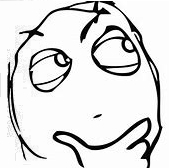
\includegraphics[width=0.3in]{why.jpg}\,}
\def\answer{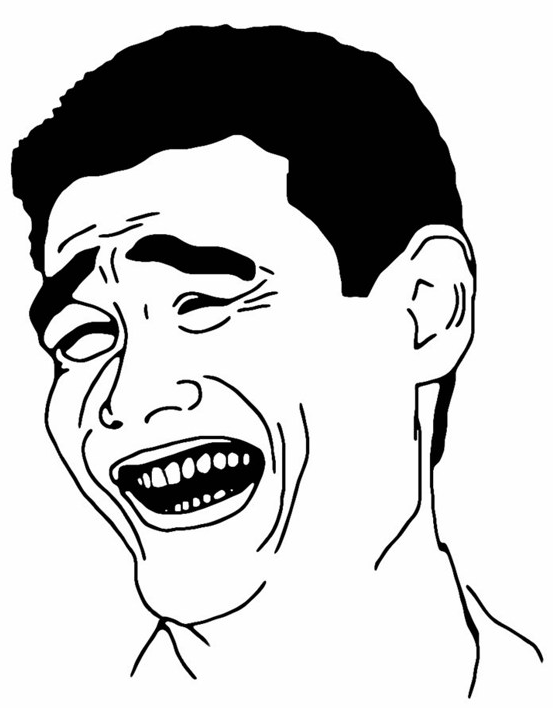
\includegraphics[width=0.3in]{baozou_haha.png}\,}
\def\wulian{
\includegraphics[width=0.18in]{emoji_wulian.jpg}}
\def\bigwulian{
\includegraphics[width=0.35in]{emoji_wulian.jpg}}
\def\bye{
\includegraphics[width=0.18in]{emoji_bye.jpg}}
\def\bigbye{
\includegraphics[width=0.35in]{emoji_bye.jpg}}
\def\huaixiao{
\includegraphics[width=0.18in]{emoji_huaixiao.jpg}}
\def\bighuaixiao{
\includegraphics[width=0.35in]{emoji_huaixiao.jpg}}
\def\jianxiao{
\includegraphics[width=0.18in]{emoji_jianxiao.jpg}}
\def\bigjianxiao{
\includegraphics[width=0.35in]{emoji_jianxiao.jpg}}
\def\haoqi{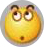
\includegraphics[width=0.18in]{emoji_haoqi.jpg}}
%% colors
\def\blacktext#1{{\color{black}#1}}
\def\bluetext#1{{\color{blue}#1}}
\def\redtext#1{{\color{red}#1}}
\def\darkbluetext#1{{\color[rgb]{0,0.2,0.6}#1}}
\def\skybluetext#1{{\color[rgb]{0.2,0.7,1.}#1}}
\def\cyantext#1{{\color[rgb]{0.,0.5,0.5}#1}}
\def\greentext#1{{\color[rgb]{0,0.7,0.1}#1}}
\def\darkgray{\color[rgb]{0.2,0.2,0.2}}
\def\lightgray{\color[rgb]{0.6,0.6,0.6}}
\def\gray{\color[rgb]{0.4,0.4,0.4}}
\def\blue{\color{blue}}
\def\red{\color{red}}
\def\orange{\color[rgb]{1.,0.8,0.}}
\def\green{\color{green}}
\def\darkgreen{\color[rgb]{0,0.4,0.1}}
\def\darkblue{\color[rgb]{0,0.2,0.6}}
\def\skyblue{\color[rgb]{0.2,0.7,1.}}
%%control
\def\diag{\mathrm{diag}\,}
\def\heaviside{\,\mathrm{h}\,}
\def\bral{\left(\begin{array}{l}}
\def\brar{\end{array}\right)}
\def\brall{\left(\begin{array}{ll}}
\def\brarr{\end{array}\right)}
\def\bralll{\left(\begin{array}{lll}}
\def\brarrr{\end{array}\right)}
\def\branchl{\left\{\begin{array}{l}}
\def\branchr{\end{array}\right.}
\def\branchll{\left\{\begin{array}{ll}}
\def\branchrr{\end{array}\right.}
\def\branchlll{\left\{\begin{array}{lll}}
\def\branchrrr{\end{array}\right.}
\def\sfgamma#1{\,\Gamma\left( #1 \right)\,}
\def\be{\begin{equation}}
\def\ee{\nonumber\end{equation}}
\def\bea{\begin{eqnarray}}
\def\eea{\nonumber\end{eqnarray}}
\def\bch{\begin{CJK}{UTF8}{gbsn}}
\def\ech{\end{CJK}}
\def\bitem{\begin{itemize}}
\def\eitem{\end{itemize}}
\def\bcenter{\begin{center}}
\def\ecenter{\end{center}}
\def\bex{\begin{minipage}{0.2\textwidth}
\includegraphics[width=0.6in]{jugelizi.png}\end{minipage}\begin{minipage}{0.76\textwidth}}
\def\eex{\end{minipage}}
\def\chtitle#1{\frametitle{\bch#1\ech}}
\def\bmat#1{\left(\begin{array}{#1}}
\def\emat{\end{array}\right)}
\def\bcase#1{\left\{\begin{array}{#1}}
\def\ecase{\end{array}\right.}
\def\bmini#1{\begin{minipage}{#1\textwidth}}
\def\emini{\end{minipage}}
\def\tbox#1{\begin{tcolorbox}#1\end{tcolorbox}}
\def\pfrac#1#2#3{\left(\frac{\partial #1}{\partial #2}\right)_{#3}}
\def\res#1#2{\,\mathrm{res}\,#1\left(#2\right)\,}
\def\newt#1#2{\left(\begin{array}{c}#1\\ #2\end{array}\right)}
\def\reof#1{\,\mathrm{Re}{\left(#1\right)\,}}
\def\imof#1{\,\mathrm{Im}{\left(#1\right)\,}}
\def\Arg#1{\,\mathrm{Arg}\,#1\,}
%%symbols
\def\intfull{\int_{-\infty}^\infty}
\def\inthalf{\int_0^\infty}
\def\bropt{\,(\ \ \ )}
\def\sech{\mathrm{sech}\,}
\def\csch{\mathrm{csch}\,}
\def\asinh{\mathrm{asinh}\,}
\def\acosh{\mathrm{acosh}\,}
\def\sone{$\star$}
\def\stwo{$\star\star$}
\def\sthree{$\star\star\star$}
\def\sfour{$\star\star\star\star$}
\def\sfive{$\star\star\star\star\star$}
\def\rint{{\int_\leftrightarrow}}
\def\roint{{\oint_\leftrightarrow}}
\def\stdHf{{\textit{\r H}_f}}
\def\deltaH{{\Delta \textit{\r H}}}
\def\ii{{\dot{\imath}}}
\def\skipline{{\vskip0.1in}}
\def\skiplines{{\vskip0.2in}}
\def\lagr{{\mathcal{L}}}
\def\hamil{{\mathcal{H}}}
\def\vecT{{\mathbf{T}}}
\def\vecN{{\mathbf{N}}}
\def\vecB{{\mathbf{B}}}
\def\vecv{{\mathbf{v}}}
\def\vecr{{\mathbf{r}}}
\def\vecf{{\mathbf{f}}}
\def\vecg{{\mathbf{g}}}
\def\vecupsilon{{\mathbf{\upsilon}}}
\def\vecu{{\mathbf{u}}}
\def\vecj{{\mathbf{j}}}
\def\vecx{{\mathbf{x}}}
\def\vecy{{\mathbf{y}}}
\def\vecz{{\mathbf{z}}}
\def\veck{{\mathbf{k}}}
\def\vecp{{\mathbf{p}}}
\def\vecn{{\mathbf{n}}}
\def\vecA{{\mathbf{A}}}
\def\vecP{{\mathbf{P}}}
\def\vecsigma{{\mathbf{\sigma}}}
\def\hatJn{{\hat{J_\vecn}}}
\def\hatJx{{\hat{J_x}}}
\def\hatJy{{\hat{J_y}}}
\def\hatJz{{\hat{J_z}}}
\def\hatj#1{\hat{J_{#1}}}
\def\hatphi{{\hat{\phi}}}
\def\hatq{{\hat{q}}}
\def\hatpi{{\hat{\pi}}}
\def\vel{\upsilon}
\def\Dint{{\mathcal{D}}}
\def\adag{{\hat{a}^\dagger}}
\def\bdag{{\hat{b}^\dagger}}
\def\cdag{{\hat{c}^\dagger}}
\def\ddag{{\hat{d}^\dagger}}
\def\hata{{\hat{a}}}
\def\hatb{{\hat{b}}}
\def\hatc{{\hat{c}}}
\def\hatd{{\hat{d}}}
\def\hatD{{\,\hat{D}}}
\def\hatN{{\hat{N}}}
\def\hatH{{\hat{H}}}
\def\hatp{{\hat{p}}}
\def\Fup{{F^{\mu\nu}}}
\def\Fdown{{F_{\mu\nu}}}
\def\newl{\nonumber \\}
\def\vece{\mathrm{e}}
\def\calM{{\mathcal{M}}}
\def\calT{{\mathcal{T}}}
\def\calR{{\mathcal{R}}}
\def\barpsi{\bar{\psi}}
\def\baru{\bar{u}}
\def\barv{\bar{\upsilon}}
\def\qeq{\stackrel{?}{=}}
\def\ftf{\stackrel{\mathcal{FT}}{\Longrightarrow}}
\def\ftb{\stackrel{\mathcal{FT}}{\Longleftarrow}}
\def\ftfb{\stackrel{\mathcal{FT}}{\Longleftrightarrow}}
\def\ltf{\stackrel{\mathcal{LT}}{\Longrightarrow}}
\def\ltb{\stackrel{\mathcal{LT}}{\Longleftarrow}}
\def\ltfb{\stackrel{\mathcal{LT}}{\Longleftrightarrow}}
\def\torder#1{\mathcal{T}\left(#1\right)}
\def\rorder#1{\mathcal{R}\left(#1\right)}
\def\contr#1#2{\contraction{}{#1}{}{#2}#1#2}
\def\trof#1{\mathrm{Tr}\left(#1\right)}
\def\trace{\mathrm{Tr}}
\def\comm#1{\ \ \ \left(\mathrm{used}\ #1\right)}
\def\tcomm#1{\ \ \ (\text{#1})}
\def\slp{\slashed{p}}
\def\slk{\slashed{k}}
\def\calp{{\mathfrak{p}}}
\def\veccalp{\mathbf{\mathfrak{p}}}
\def\Tthree{T_{\tiny \textcircled{3}}}
\def\pthree{p_{\tiny \textcircled{3}}}
\def\dbar{{\,\mathchar'26\mkern-12mu d}}
\def\erf{\mathrm{erf}}
\def\const{\mathrm{const.}}
\def\pheat{\pfrac p{\ln T}V}
\def\vheat{\pfrac V{\ln T}p}
%%units
\def\fdeg{{^\circ \mathrm{F}}}
\def\cdeg{^\circ \mathrm{C}}
\def\atm{\,\mathrm{atm}}
\def\angstrom{\,\text{\AA}}
\def\SIL{\,\mathrm{L}}
\def\SIkm{\,\mathrm{km}}
\def\SIyr{\,\mathrm{yr}}
\def\SIGyr{\,\mathrm{Gyr}}
\def\SIV{\,\mathrm{V}}
\def\SImV{\,\mathrm{mV}}
\def\SIeV{\,\mathrm{eV}}
\def\SIkeV{\,\mathrm{keV}}
\def\SIMeV{\,\mathrm{MeV}}
\def\SIGeV{\,\mathrm{GeV}}
\def\SIcal{\,\mathrm{cal}}
\def\SIkcal{\,\mathrm{kcal}}
\def\SImol{\,\mathrm{mol}}
\def\SIN{\,\mathrm{N}}
\def\SIHz{\,\mathrm{Hz}}
\def\SIm{\,\mathrm{m}}
\def\SIcm{\,\mathrm{cm}}
\def\SIfm{\,\mathrm{fm}}
\def\SImm{\,\mathrm{mm}}
\def\SInm{\,\mathrm{nm}}
\def\SImum{\,\mathrm{\mu m}}
\def\SIJ{\,\mathrm{J}}
\def\SIW{\,\mathrm{W}}
\def\SIkJ{\,\mathrm{kJ}}
\def\SIs{\,\mathrm{s}}
\def\SIkg{\,\mathrm{kg}}
\def\SIg{\,\mathrm{g}}
\def\SIK{\,\mathrm{K}}
\def\SImmHg{\,\mathrm{mmHg}}
\def\SIPa{\,\mathrm{Pa}}
%page
\def\secpage#1#2{\begin{frame}\bcenter{\bf \Huge #1} \ecenter \skipline \tbox{\bcenter #2 \ecenter}\end{frame}}
\def\append#1#2{\secpage{附录#1}{#2}}
\def\thinka#1{\begin{frame}\frametitle{思考题}\bcenter\lfig{0.4}{think0.jpg}  \skipline #1 \ecenter\end{frame}}
\def\thinkb#1{\begin{frame}\frametitle{思考题}\bcenter\lfig{0.5}{think1.jpg}  \skipline #1 \ecenter\end{frame}}
\def\thinkc#1{\begin{frame}\frametitle{思考题}\bcenter\lfig{0.5}{think2.jpg}  \skipline #1 \ecenter\end{frame}}
\def\thinkd#1{\begin{frame}\frametitle{思考题}\bcenter\lfig{0.5}{think3.jpg}  \skipline #1 \ecenter\end{frame}}
\def\thinke#1{\begin{frame}\frametitle{思考题}\bcenter\lfig{0.5}{think4.jpg}  \skipline #1 \ecenter\end{frame}}
\def\thinkf#1{\begin{frame}\frametitle{思考题}\bcenter\lfig{0.5}{think5.jpg}  \skipline #1 \ecenter\end{frame}}
\def\schw{ds^2 = \left(1-\frac{2GM}{r}\right)dt^2 - \left(1-\frac{2GM}{r}\right)^{-1} dr^2 - r^2\left(d\theta^2 + \sin^2\theta d\phi^2\right)}

\input{titlepage.tex}
  \date{}
  \begin{document}
  \bch
\tpage{4}{Gaussian Curvature}


\secpage{课前小练习}{两个二次型之比}

\begin{frame}
  \frametitle{按照惯例,先回忆下美好的线性代数……}

  \addfig{0.8}{think5.jpg}
  
  设矩阵 $A,B$ 都是 $n\times n$ 的实对称矩阵,且  $A$ 是正定的。
  
对$n\times 1$ 的非零列向量 $\vecx$,定义
$$ f(\vecx) = \frac{\vecx^TB\vecx}{\vecx^TA\vecx}.$$
 $f(\vecx)$ 的取值范围是怎样的?取到最小值和最大值的条件分别是什么?
\end{frame}


\begin{frame}
  令 $\vecy = A^{1/2}\vecx $, $C = A^{-1/2} B A^{-1/2}$,则  
  $$ f(x) = \frac{\vecy^TC\vecy}{\vecy^T\vecy} $$
  在 $C$ 的本征矢为基的空间看,这个表达式只是 $C$ 的各个本征值的加权平均,权重均非负。所以取值范围为
  $\left[\lambda_{\min}, \lambda_{\max}\right]$。这里的 $\lambda_{\min},\lambda_{\max}$ 分别是 $C$ 的最小和最大的本征值。取到最小值和最大值的条件分别是 $\vecy$ 为 $\lambda_{\min},\lambda_{\max}$ 对应的本征矢。


  \skiplines
  
  {\scriptsize 一个实对称矩阵 $A$ 的解析函数 $f(A)$ 可以这样计算:把矩阵正交对角化 $A = R\Lambda R^T$,这里的 $R^TR=I$, $\Lambda=\diag(\lambda_1,\lambda_2,\ldots)$。然后对任意非负整数 $n$,有
    $$A^n = R\Lambda R^T R\Lambda R^T\ldots R\Lambda R^T = R\Lambda^n R^T = R\,\diag(\lambda_1^n, \lambda_2^n, \ldots) R^T.$$
    于是对任何可以局域地展成幂级数的函数 $f$,可以认为
    $$ f(A) = R\, \diag(f(\lambda_1), f(\lambda_2), \ldots) R^T.$$
    显然 $f(A)$ 仍然是对称矩阵。
  }
\end{frame}

\secpage{描述曲面的弯曲程度}{药丸}


\begin{frame}
  我们曾经用一段近似圆弧来描述曲线的弯曲程度。曲线的曲率就是圆弧半径的倒数。


  \skiplines
  
  那么曲面的弯曲程度是不是可以用一个近似球面来描述?(并把球面半径倒数称为曲率?)
  
\end{frame}


\begin{frame}
  答案是 NO。

  请凝视下面的药丸(特别是它的侧边)三秒钟,不解释。
  
  \addfig{2}{yaowan.jpg}
\end{frame}


\begin{frame}

  结论:三维空间里的曲面的局域近似不能用球面,要用药丸。

  \addfig{2}{yaowan.jpg}

  观察这个药丸的侧边,设曲面上的沿着两个正交的方向的曲线(近似圆弧)的曲率分别为
  $\kappa_{\min}, \kappa_{\max}$。沿着其他方向的曲线的曲率似乎介于两者之间。下面我们就来就如何计算 $\kappa_{\min}, \kappa_{\max}$ 以及任意方向的曲线的曲率进行一波推导。

  为此,我们先引入一波奇怪的符号……
\end{frame}

\secpage{一大波奇怪的符号来袭……}{感到呼吸困难}


\begin{frame}
  \frametitle{奇怪的右上指标}
  毕竟我们最后是要讨论四维的弯曲时空。为了能和更高维度的弯曲空间接轨,我们有必要从现在开始就使用一些不很依赖于维度的符号。

  \skipline

  例如,我们要把描述曲面的 $u, v$, 换成 $u^1, u^2$。


  \addfig{1.2}{zhongdian2.jpg}
  
 {\bf $u^1, u^2$ 不是 $u$ 的一次方,二次方的意思。它们仅仅表示曲面上的第一个和第二个变量(爬虫用的世界坐标)。}

\end{frame}


\begin{frame}
  \frametitle{关于变量指标在右上这件事情的Q\&A}
  \question 我看到 $u^1, u^2$ 这样的符号感到很不适,需要服用双黄连吗?
  
  \answer 建议上呼吸机。
\end{frame}


\begin{frame}
  \frametitle{关于变量指标在右上这件事情的Q\&A}
  \question 第二个变量的平方怎么写?
  
  \answer $u^2u^2$ (这个是否让你感觉更糟糕\huaixiao) 或者 $\left(u^2\right)^2$。但大多数情况下我们不需要写这个东西。
\end{frame}


\begin{frame}
  \frametitle{关于变量指标在右上这件事情的Q\&A}
  \question 怎么区分 $u$ 的平方和 $u^2$?
  
  \answer $u$ 的平方是啥意思?

  \question $u = (u^1, u^2)$的话,$u$ 的平方就是: $ (u^1)^2+(u^2)^2$

  \answer 看,你已经写出来了!

  (不过,这个表达式仍然不怎么常用,因为这样的 $u$ 平方的定义只对欧式空间的直角坐标成立。我们以后会给出任意空间内 $u$ 的平方的含义,并给出新的写法。)
\end{frame}


\begin{frame}
  \frametitle{曲面的第一基本形式}
  $$ d\vecx^2  =
  \begin{pmatrix}
    du^1 &    du^2
  \end{pmatrix}
  \begin{pmatrix}
    g_{11} &   g_{12} \\
    g_{21} & g_{22}
  \end{pmatrix}
  \begin{pmatrix}
    du^1 \\
    du^2
  \end{pmatrix}  
  =  \sum_{i=1}^2\sum_{j=1}^2 g_{ij}du^i du^j.$$
  这里度规矩阵 $g_{ij}$ ($i,j=1,2$)定义为
  $$g_{ij} = \frac{\partial\vecx}{\partial u^i}\cdot\frac{\partial\vecx}{\partial u^j}.$$
  注意,我们把 $g_{ij}$ 里的 $i, j$ 都写成了下标。这是因为等号右边的上标 $i, j$ 都在分母——当把上标放到分母,它会变成下标;反之亦然。
\end{frame}

\begin{frame}
  \frametitle{爱因斯坦求和规则}
  当爱因斯坦研究广义相对论时,写着一堆求和号的表达式满天乱飞。为了节省笔墨保护森林,他提出一个约定:{\blue 如果一个指标在上标和下标中各出现一次,那么就默认对它进行求和。}

  \addfig{2}{einstein.jpg}
  
  这样第一基本形式可以写成:
  $$ d\vecx^2 = g_{ij}du^i du^j.$$
  这里的 $i$, $j$ 都按约定默认进行求和。
\end{frame}


\begin{frame}
  \frametitle{曲面的第二基本形式}
  $$\vecn\cdot d^2\vecx = - d\vecn\cdot d\vecx = \beta_{ij}du^i du^j.$$
  等式右边同样按爱因斯坦求和规则对 $i, j$ 进行求和。

  这里的
  $$ \vecn = \frac{\frac{\partial\vecx}{\partial u^1}\times \frac{\partial\vecx}{\partial u^2}}{\lvert\frac{\partial\vecx}{\partial u^1}\times \frac{\partial\vecx}{\partial u^2}\rvert}. $$
  
  $$ \beta_{ij} = \vecn \cdot \frac{\partial^2\vecx}{\partial u^i \partial u^j} = - \frac{\partial \vecn}{\partial u^i} \cdot \frac{\partial \vecx}{\partial u^j} = - \frac{\partial \vecx}{du^i} \cdot \frac{\partial \vecn}{\partial u^j}$$
\end{frame}

\begin{frame}
  \frametitle{偏导用逗号}
  在不至引起混淆的情况下,我们还约定,对 $u^i$ 的偏导数用下标 $_{, i}$ 来表示。

  \skipline
  
  这样

  $$g_{ij} = \vecx_{, i} \cdot \vecx_{,j}$$

  $$\beta_{ij} = \vecn \cdot \vecx_{, i, j} = - \vecn_{, i} \cdot \vecx_{, j} = - \vecx_{, i}\cdot \vecn_{, j} $$  
 
\end{frame}


\begin{frame}
  好了,符号介绍完了。

  \skiplines
  
  戴上你的呼吸机,我们要开始起飞了——
\end{frame}


\begin{frame}
  \frametitle{曲面上的曲线}
  曲面上的曲线可以写成 $ \vecx\left(u^1(s), u^2(s)\right)$,这里 $s$ 为弧长参数。

  \skipline
  
  曲线的单位切向量
  $$\frac{d\vecx}{ds} = \vecx_{,i} \frac{du^i}{ds}. $$
  曲线的曲率向量
  $$\frac{d^2\vecx}{ds^2} = \vecx_{,i,j} \frac{du^i}{ds}\frac{du^j}{ds} + \vecx_{, i} \frac{d^2 u^i}{ds^2}. $$
  当然,这样算出来的曲率并不代表曲面的弯曲程度,因为即使是完全没有弯曲的平面,你也可以在上面取一条曲率非零的曲线——只是,它的曲率向量会落在平面内。

  \skipline

  结论就是:曲率向量落在曲面的切向的部分都不能表征曲面的弯曲程度;曲率向量落在曲面的法向的部分才表征曲面弯曲程度。
  
\end{frame}


\begin{frame}
  \frametitle{法向曲率}
  把曲率向量投影到曲面的法向 $\vecn$ 上,得到
  $$ \vecn \cdot \frac{d^2\vecx}{ds^2} =  \beta_{ij} \frac{du^i}{ds}\frac{du^j}{ds}.$$
  (注意第二项消失是因为 $\vecn \cdot d\vecx = 0$)
  
  注意到切向的 $ds^2$ 其实就是第一基本形式 $g_{ij}du^i du^j$,上面的结果可以写成:
  $$ \vecn \cdot \frac{d^2\vecx}{ds^2} =  \frac{\beta_{ij}du^i du^j}{g_{ij}du^idu^j}.$$
  也就是说,{\blue 沿 $(du^1, du^2)$ 方向的曲线的法向曲率等于第二基本形式和第一基本形式之比。}


\end{frame}


\begin{frame}
  \frametitle{法向曲率是两个本征曲率的加权平均}
  $$ \vecn \cdot \frac{d^2\vecx}{ds^2} =  \frac{\beta_{ij}du^i du^j}{g_{ij}du^idu^j}.$$
  这个表达式,两个二次型之比,眼熟不?

  对,它就是矩阵 $C=g^{-1/2}\beta g^{-1/2}$ 的两个本征值 $\kappa_{\max}, \kappa_{\min}$ 的加权平均。

  设 $$ g^{1/2}\begin{pmatrix}du^1 \\ du^2 \end{pmatrix}$$
  和$C$ 对应于 $\kappa_{\max}, \kappa_{\min}$ 的两个本征矢之间的夹角为 $\theta$,则沿 $(du^1, du^2)$ 方向的曲线的法向曲率等于
  {\blue $$ \kappa_{\max}\cos^2\theta + \kappa_{\min}\sin^2\theta.$$}
  这个公式最早是欧拉发现的。
\end{frame}


\begin{frame}
  我们把 $C=g^{-1/2}\beta g^{-1/2}$ 的两个本征值 $\kappa_{\max}, \kappa_{\min}$ 称为曲面的两个主曲率。
  
  \addfig{2}{yaowan.jpg}

  药丸的边缘上的两个主曲率的就是正交的两条弧线的半径的倒数。
\end{frame}


\begin{frame}
  \frametitle{主曲率的计算}
  $C=g^{-1/2}\beta g^{-1/2}$  的本征值方程是
  $$  \det\left(g^{-1/2}\beta g^{-1/2} - \lambda I \right) = 0$$
  左乘  $g^{1/2}$ 右乘 $g^{1/2}$,显然不影响矩阵的零秩性,于是上式等价于
  $$ \det\left(\beta - \lambda g\right) = 0$$
  具体写出来就是
  $$ \det(g) \lambda^2 +(2g_{12}\beta_{12}-g_{11}\beta_{22}-g_{22}\beta_{11})\lambda +\det(\beta) = 0.$$
  于是根据韦达定理,有
  $$ \kappa_{\min}+\kappa_{\max} = \frac{g_{11}\beta_{22}+g_{22}\beta_{11}-2g_{12}\beta_{12}}{\det(g)}.$$
  $$ \kappa_{\min}\kappa_{\max} = \frac{\det(\beta)}{\det(g)}.$$  
\end{frame}


\begin{frame}
  \frametitle{高斯曲率}
  两个主曲率的乘积
  $$K = \kappa_{\min}\kappa_{\max} = \frac{\det(\beta)}{\det(g)}.$$
  叫做曲面的{\blue 高斯曲率}。它比两个主曲率之和 $\kappa_{\min}+\kappa_{\max} $ 要重要得多。这是为什么呢?

\end{frame}


\begin{frame}
  \frametitle{高斯曲率的重要性}
  {\small
    还记得《广义相对论》是要干啥吗?{\blue 通过第一基本形式来研究空间的弯曲性质。}

    在一维的曲线上,如果只允许在曲线上测距,则只能确定弧长变量 $s$ 而无法获得曲率或挠率的信息。曲线上的爬虫不可能通过第一基本形式来研究空间的弯曲性质。也就是说,{\blue 一维曲线没有内禀弯曲,它总是可以无伸缩地拉成一条直线。}

    二维曲面的情况则有所不同,只有像圆柱、圆锥这样的曲面才能无伸缩地拉成一个平面。圆柱、圆锥的特点是:总是有一个“直”的方向,也就是两个主曲率之一是零,或者说高斯曲率 $\kappa_{\min}\kappa_{\max} = 0$。这暗示着我们高斯曲率可能和曲面的内禀弯曲有关。而 $\kappa_{\min}+\kappa_{\max}$ 在圆柱和圆锥上均不为零,则可能对应高维空间才能看到的非内禀弯曲。 

    如果回到高斯曲率的计算公式 $K=\frac{\det(\beta)}{\det(g)}$,似乎还是需要曲面的第二基本形式(高维信息)才能计算。但是,这个结论仅对一个孤立的点成立。如果我们把不同点的第一基本形式联系起来,就会发现一个神奇的现象:高斯曲率可以完全只通过第一基本形式获得,而 $\kappa_{\min}+\kappa_{\max}$ 则不行
  }
\end{frame}


\begin{frame}
  \frametitle{高斯的脑洞}
  {\blue 高斯曲率是曲面的内禀性质,只要在曲面上测距(不需要高维的信息)就能获得。}这个美妙的结论是高斯发现的。

  \skiplines
  
  高斯的 sympy.oo 才华决定了他不会把这个结论当成一个平凡的数学结果。他指出:曲面的弯曲程度等几何性质可以限定在曲面上进行讨论。{\blue(尔等菜鸡)想象曲面放在一个三维或更高维的空间里是完全没有必要的步骤。}

  \addfig{1.5}{jiangweidaji.jpg}

  
\end{frame}


\begin{frame}
  下一讲我们将讨论: 如何只用曲面第一基本形式推出高斯曲率
  
  \addfig{1}{caigou.jpg}
  

\end{frame}

\ech
\end{document}
